%
% This docuement is based on the Insight Journal Template.
% https://github.com/InsightSoftwareConsortium/InsightJournalTemplate/tree/ModularTemplate
% 4555fc04b105b11f06dc302b76bf09c27e50727d

\documentclass{InsightArticle}

\usepackage[dvips]{graphicx}
\usepackage{listings}
%  hyperref should be the last package to be loaded.
\usepackage[dvips,
bookmarks,
bookmarksopen,
backref,
colorlinks,linkcolor={blue},citecolor={blue},urlcolor={blue},
]{hyperref}

\lstset{ %
language=C++,                % choose the language of the code
basicstyle=\footnotesize,       % the size of the fonts that are used for the code
numbers=left,                   % where to put the line-numbers
numberstyle=\footnotesize,      % the size of the fonts that are used for the line-numbers
stepnumber=1,                   % the step between two line-numbers. If it is 1 each line will be numbered
numbersep=5pt,                  % how far the line-numbers are from the code
backgroundcolor=\color{white},  % choose the background color. You must add \usepackage{color}
showspaces=false,               % show spaces adding particular underscores
showstringspaces=false,         % underline spaces within strings
showtabs=false,                 % show tabs within strings adding particular underscores
frame=single,           % adds a frame around the code
tabsize=2,          % sets default tabsize to 2 spaces
captionpos=b,           % sets the caption-position to bottom
breaklines=true,        % sets automatic line breaking
breakatwhitespace=false,    % sets if automatic breaks should only happen at whitespace
escapeinside={\%*}{*)}          % if you want to add a comment within your code
}


\title{BinShrink: A multi-resolution filter with cache efficient averaging. }

\newcommand{\IJhandlerIDnumber}{0}

\release{0.00}

% At minimum, give your name and an email address.  You can include a
% snail-mail address if you like.
\author{Bradley C. Lowekamp$^{1}$ and David T. Chen$^{1}$}
\authoraddress{$^{1}$National Library Of Medicine}

\begin{document}

%
% Add hyperlink to the web location and license of the paper.
% The argument of this command is the handler identifier given
% by the Insight Journal to this paper.
%
\IJhandlefooter{\IJhandlerIDnumber}


\ifpdf
\else
   %
   % Commands for including Graphics when using latex
   %
   \DeclareGraphicsExtensions{.eps,.jpg,.gif,.tiff,.bmp,.png}
   \DeclareGraphicsRule{.jpg}{eps}{.jpg.bb}{`convert #1 eps:-}
   \DeclareGraphicsRule{.gif}{eps}{.gif.bb}{`convert #1 eps:-}
   \DeclareGraphicsRule{.tiff}{eps}{.tiff.bb}{`convert #1 eps:-}
   \DeclareGraphicsRule{.bmp}{eps}{.bmp.bb}{`convert #1 eps:-}
   \DeclareGraphicsRule{.png}{eps}{.png.bb}{`convert #1 eps:-}
\fi


\maketitle


\ifhtml
\chapter*{Front Matter\label{front}}
\fi

% The abstract should be a paragraph or two long, and describe the
% scope of the document.
\begin{abstract}
\noindent
We present a new filter for the Insight Toolkit (ITK) for reducing the
resolution of an image by an integer factor while averaging called
\textit{BinShrink}. This filter provides a new level of performance to
ITK for reducing resolution and noise present in an image. The filter
supports streaming, multi-threading and most of ITK's pixel types
including scalars, \textit{Vector}s,
\textit{SymmetricSecondRankTensor}s, and \textit{RGBPixel}s.

\end{abstract}

\IJhandlenote{\IJhandlerIDnumber}

\tableofcontents

% don't like
This ``binning'' algorithm is commonly used in processing of high
resolution electron microscopy image. It's available in such packages
as The Boulder Laboratory for 3-D Electron Microscopy of Cell's
IMOD\cite{IMOD}, \cite{bsoft2007}.
Multi-resolution

Why is this filter useful?


This document describes a new algorithm not currently in
ITK\cite{ITKSoftwareGuide}.

\section{Implementation}

The algorithm implmentated in the \textit{BinShrink} filter can be
described with (Eqn (\ref{eqn:Algo})) for the 2D case.
\begin{equation}
\label{eqn:Algo}
\mathsf{I}_{out}(x_o,x_1) = \frac{\sum_{i=0}^{f_0}\sum_{j=0}^{f_1}\mathsf{I}_{in}(f_0 x_o+i,f_1 x_1+j)}{f_0 f_1}
\end{equation}

The output image is only defined when all the required input image
pixels are defined. The vector variable $\mathbf{\overline{f}}$ is a user defined
shrink factor.

The method operates on a local input and output region making the
filter appropriate for streaming. Also the only operations required are
pixel wise addition and division by a scalar, so that it can readily
work with a wide variety of pixel types.

\subsection{Geometry}

The geometry of an image includes it's pixel spacing, origin, and
image orientation. For this filter there is no change in the orientation but the
spacing is scaled by the shrink factor. However, there is some
complication when defining the origin. When the input image size is
not evenly dividable by the shrinking factors a choice on how to
``round'' the pixels location needs to be made. We have chosen to maintain the physical
location for the image signal and truncate the odd pixels at the
boundaries. As ITK image can have non-zero starting indexes, we define
the output origin pixel must lay on the same lower boundary as the
input, and the origin must be adjusted accordingly (See figure \ref{fig:PixelGrid}).

\begin{figure}
  \centering
  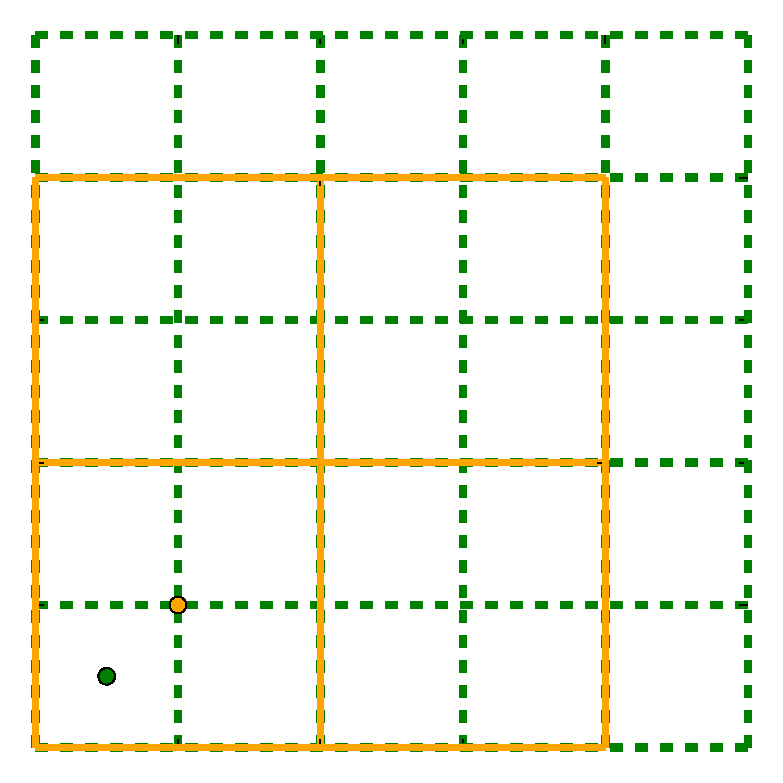
\includegraphics[width=0.4\linewidth]{images/pixelgrid}
  \itkcaption{This represents the change in geometry from a 5x5 image
    binned by a factor of 2x2. The green dotted lines is the input
    image. The yellow grid is the result of the filter. The points
    represent the respective origins.}
  \label{fig:PixelGrid}
\end{figure}

While this approach maintains the physical location of the image
signal to does not maintain neither the full extent nor the
center of the image. Therefore for algorithms such an image pyramids or certain
neuro-imaging analysis, this method may not be appropriate or
insurances need to be made such that the input size is divisible by the shrink factor.

\subsection{Initial Implementation}

We have inlcuded the initial implementation of the filter in the
submittion for performance comparison purposes and have named it
\textit{BinShrink2}. The above description of geometry applies only to the
\textit{BinShrink} filter. The original \textit{BinShrink2} was
derived from ITK's \textit{Shrink} filter, which has different
geomentry then described above. The original \textit{BinShrink2}
follows the same geometry as the \textit{Shrink} filter.

This original implementation used ITK's conventional
\textit{NeighborhoodIterator} to average the input for each output
(See Listing \ref{lst:01}).

\begin{lstlisting}[label=lst:01, caption={A selected section of code
      from \textit{BinShrink2} filter using the neighborhood iterator.}]
while ( !outIt.IsAtEnd() )
  {
  outputIndex = outIt.GetIndex();

  inputIndex = outputIndex * factorSize + offsetIndex;

  inputIt.SetLocation( inputIndex );

  AccumulatePixelType sum = NumericTraits<AccumulatePixelType>::Zero;
  typename ConstNeighborhoodIteratorType::ConstIterator ci = inputIt.Begin();

  for (ci.GoToBegin(); !ci.IsAtEnd(); ++ci)
    {
    sum += AccumulatePixelType( ci.Get() );
    }
  sum = sum / double( inputIt.GetActiveIndexListSize() );

  outIt.Set( sum );
  ++outIt;
  }
\end{lstlisting}


\subsection{Optimization}

The implementation we suggest for inclusion in ITK is the
\textit{BinShrink}, which follows the geomentry specifically described
above and is not derived from the \textit{ShrinkFilter}. The initial
implementation accesses the memory in an incoherent fashion based on
the input neighborhood. However, it is faster to access memory in a
linear and coherent fashion. This lead to the goal of accessing the
input image on a per scan-line basis, and operating the
averaging on scan-lines as opposed to pixels. By utilizing ITK's
\textit{ScanlineIteators}, we improved the algorithm to work on a
scan-lines for the inner most loops (See Listing \ref{lst:01}).

\begin{lstlisting}[label=lst:02, caption={A selection of code from the
  \textit{BinShrink} filter demonstrating scan-line averaging.}]
while ( !outputIterator.IsAtEnd() )
  {
  const OutputIndexType outputIndex = outputIterator.GetIndex();

  typename std::vector<OutputOffsetType>::const\_iterator offset = offsets.begin();
  const InputIndexType startInputIndex = outputIndex * factorSize;

  while ( ++offset != offsets.end() )
    {
    inputIterator.SetIndex( startInputIndex+*offset );

    for( size\_t i = 0; i < ln; ++i )
      {
      for( size\_t j = 0; j < factorSize[0]; ++j)
        {
        accBuffer[i] += inputIterator.Get();
        ++inputIterator;
        }
      }
    }

    for ( size\_t j = 0; j <ln;++j)
    {
      accBuffer[j] = accBuffer[j] * inumSamples;
      outputIterator.Set( static\_cast<OutputPixelType>(accBuffer[j]) );
      ++outputIterator;
    }

    outputIterator.NextLine();
  }
\end{lstlisting}

\section{Results}

To test our BinShrink filter we have used a synthetic function
created by Marschner and Lobb\cite{MarschnerL94}, along with additive
noise to create test volume images. This function is often used to
evaluate volume rendering reconstruction filters. We have rendered it
into a 128 pixel cubic volume such that the majority of the frequencies in
the function are sampled just above 4 times the Nyquist frequency. Such an image
makes for a challenging theoretical data set when the shrinking factor is also
4.

The code used to generate these images was written in Python with
SimpleITK. The original Marshner-Lobb volume was normalized with the
\textit{Normalize} filter so that the volume had a mean
of 0 and a standard deviation of 1. Then Gaussian distributed random
noise was added with a 0 mean and a sigma to achieve the targeted
signal to noise ratio. After the shrinking operation was performed,
the volume was again normalized for contrast. Then the center slice
was extracted and tiled. Finally it was colorized by the
\textit{ScalarToRGBColormap} filter\cite{Tustison2009}.

We examined the results of the \textit{BinShrink} filter by varying the
signal to noise ratio in our Marshnel-Lobb test image and then shrinking those noisy
images by factors of 2 and 4 (See figure
\ref{fig:BinShrinkComparison}). For comparison we also used the
\textit{SmoothingRecusiveGaissian} filter in conjunction with the
\textit{Shrink} filter on the same test noisy images.  We set \textit{sigma} of the
smoothing Gaussian kernel at 0.7 times the shrink factor.

[NEED TO TALK ABOUT ALIASING AND IMAGE QUALITY, SINCE IT'S MENTIONED IN THE CONCLUSION]

\begin{figure}
  \centering
  
\includegraphics[width=0.4\linewidth]{images/binshrink_hot.png}
  \caption[Registration Framework Components]{The basic components of the
    registration framework are two input images, a transform, a metric, an
    interpolator and an optimizer.}
  \label{fig:BinShrinkComparison}
\end{figure}

\begin{figure}
  \centering
  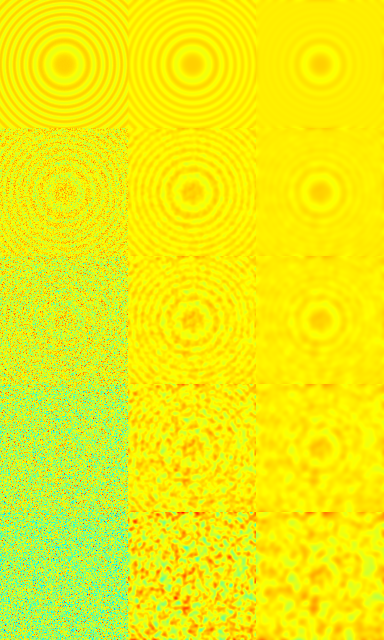
\includegraphics[width=0.4\linewidth]{images/gaussianshrink_hot.png}
  \caption[Registration Framework Components]{The basic components of the
    registration framework are two input images, a transform, a metric, an
    interpolator and an optimizer.}
  \label{fig:GaussianShrinkComparison}
\end{figure}

\subsection{Performance}

To analyze the performance of our bin shrinking methods we compare them
against similar processes which can be performed in ITK with other pairs of filters.

Running a \textit{Mean} filter followed by a \textit{Shrink} filter is a
close approximation to \textit{BinShrink}. The
\textit{Mean} filter computes an average for each input pixel's
neighborhood in a brute force fashion. This approach wastes computation on input
pixels that are dropped by the \textit{Shrink} filter.

Using a Gaussian kernel to reduce aliasing is an alternative to the box
kernel implicitly used with the \textit{BinShrink} filter. Gaussian filtering can be
performed in constant time and independent of the size of the Gaussian with
the \textit{SmoothingRecusiveGaussian} filter.

We generated a 384 pixel cubic image of Gaussian distributed noise for
performance evaluation. We set the number of threads used to be
16. Utilizing SimpleITK and Python's
\textit{timeit} module, we report the median of 3 runs for each
algorithm across varying shrink factors (See Figure
\ref{fig:ShrinkPerformance}).  The image size, the number of threads,
and the shrink factors were carefully chosen such that the output
image was always evenly divided for multi-threading. As expected the
\textit{Mean} approach suffers from exponential cost as a function of
shrink size, while the
\textit{SmoothingRecursiveGaussian} method remains constant. The
\textit{BinShrink2} implementation only touches each input pixel once,
but it also suffers from exponential growth likely due to its memory
access pattern being inefficient and not cache coherent. On the other
hand the \textit{BinShrink} implementation execution time decreases as
the shrink factor increases.

\begin{figure}
  \centering
  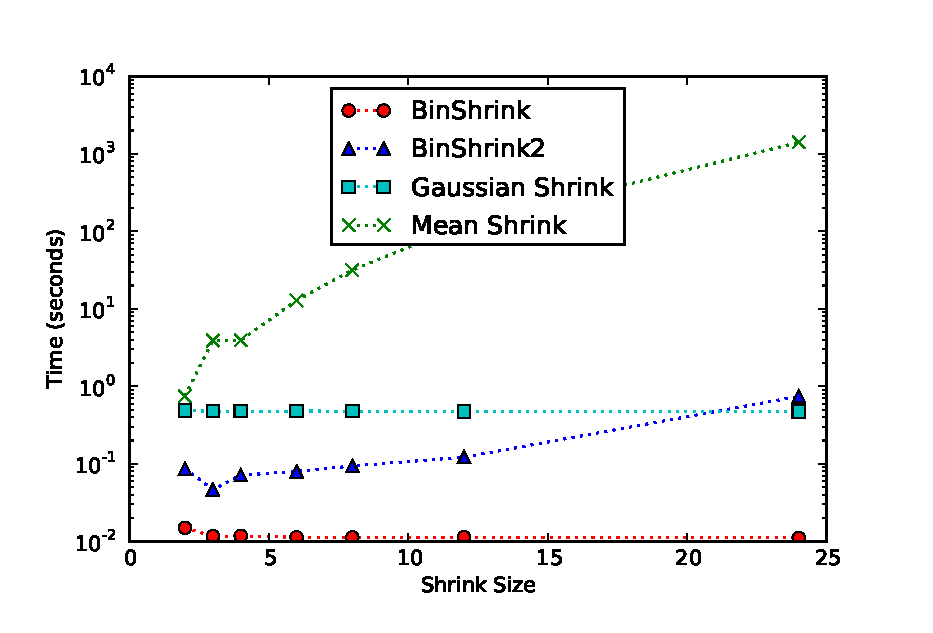
\includegraphics[width=0.8\linewidth]{images/shrink_time}
  \itkcaption{Performance}
  \label{fig:ShrinkPerformance}
\end{figure}

\begin{table}
\begin{center}
\begin{tabular}{l|*{7}{c}r}
Algorithm & \multicolumn{7}{c}{Shrink Factor} \\
  &            2 & 3 & 4 & 6 & 8 & 12 & 24 \\
\hline
BinShrink &     0.0149s & 0.0116s & 0.0118s & 0.0113s & 0.0112s & 0.0113s & 0.0110s\\
BinShrink2 &    0.0862s & 0.0465s & 0.0714s & 0.0797s & 0.0940s & 0.1217s & 0.7451s\\
GaussianShrink &0.4850s & 0.4779s & 0.4778s & 0.4803s & 0.4791s & 0.4752s & 0.4767s\\
MeanShrink &    0.7440s & 3.9093s & 3.9264s & 12.818s & 31.602s & 121.80s & 1412.3s\\
\end{tabular}
\itkcaption{Performance}
\label{tab:ShrinkPerformance}
\end{center}
\end{table}

This is quite the interesting case for analyzing the difference
between the \textit{BinShrink} and \textit{BinShrink2}. TODO after
final numbers...

\section{Conclusion}

We have demonstrated that the \textit{BinShrink} filter is a fast
filter to be used for multi-resolutional work. Based on the resulting
images, it may not always be the best methods for image quality as it
may result in aliasing. However, features such as wide pixel type
support and streaming make it quite practical for working with large
data sets.


\bibliographystyle{plain}
\bibliography{BinShrink}


\end{document}
